\documentclass[a4paper, 12pt]{article}

\usepackage{iftex}
\ifPDFTeX
    % pdfLaTeX: кириллица через T2A
    \usepackage[T1, T2A]{fontenc}
    \usepackage[utf8]{inputenc}
    \usepackage[english, russian]{babel}
\else
    % XeLaTeX / LuaLaTeX: нужен шрифт с кириллицей (берём первый найденный)
    \usepackage{fontspec}
    \usepackage[english, russian]{babel}
    % Windows/macOS: Times New Roman и Courier New; Linux: Liberation или DejaVu
    \IfFontExistsTF{Times New Roman}{\setmainfont{Times New Roman}}{%
    \IfFontExistsTF{Liberation Serif}{\setmainfont{Liberation Serif}}{%
    \setmainfont{DejaVu Serif}}}
    \IfFontExistsTF{Courier New}{\setmonofont{Courier New}}{%
    \IfFontExistsTF{Liberation Mono}{\setmonofont{Liberation Mono}}{%
    \setmonofont{DejaVu Sans Mono}}}
\fi
\usepackage{graphicx}
\usepackage{float}
\usepackage{geometry}
\usepackage{amsmath}
\usepackage{amsfonts}
\usepackage{booktabs}
\usepackage[dvipsnames]{xcolor}
\usepackage[colorlinks]{hyperref}
\usepackage{indentfirst}
\usepackage{listings}
\usepackage{src/title}

\geometry{left=2cm, right=2cm, bottom=2cm, top=2cm}

\hypersetup{
    linkcolor=blue,
    filecolor=magenta,
    urlcolor=cyan
}

\definecolor{codegreen}{rgb}{0,0.6,0}
\definecolor{codegray}{rgb}{0.5,0.5,0.5}
\definecolor{codepurple}{rgb}{0.58,0,0.82}
\definecolor{backcolour}{rgb}{0.95,0.95,0.92}

\lstdefinestyle{codestyle}{
    backgroundcolor=\color{backcolour},
    commentstyle=\color{codegreen},
    keywordstyle=\color{magenta},
    numberstyle=\tiny\color{codegray},
    stringstyle=\color{codepurple},
    basicstyle=\ttfamily\footnotesize,
    breakatwhitespace=false,
    breaklines=true,
    captionpos=b,
    keepspaces=true,
    numbers=left,
    numbersep=5pt,
    showspaces=false,
    showstringspaces=false,
    showtabs=false,
    tabsize=2
}
\lstset{style=codestyle}
\lstset{extendedchars=\true}

\newcommand{\vect}[2]{\begin{pmatrix}#1\\#2\end{pmatrix}}
\DeclareMathOperator{\rank}{rank}
\DeclareMathOperator{\tr}{tr}

\title{
    Практическая линейная алгебра — Лабораторная работа №2
}

\author{%
    Ануфриев Андрей Сергеевич (465029)\\
    Бахуров Николай Алексеевич (504862)\\
    Раджапов Фёдор Сергеевич (502544)%
}

\supervisor{Зарина Ольга Андреевна}

\abstract{
    В работе исследованы линейные преобразования плоскости, задаваемые матрицами $2 \times 2$. Для параметров $a=3$, $b=4$, $c=2$, $d=5$ построены матрицы отражений, проекции, поворотов, композиций и отображений с заданными свойствами собственных векторов, получены общие классы таких матриц. Выполнен анализ образа, ядра, собственных чисел и векторов, определителей и свойств матриц. Все матрицы проверены численно, образы многоугольника и окружности визуализированы на Python.
}

\keywords{
    линейные преобразования; матрицы $2\times 2$; собственные векторы; определитель; жорданова форма; визуализация
}

\date{2026-10-01}

\begin{document}
    \maketitle
    \tableofcontents
    \newpage

    \section{Постановка задачи}
    Любая матрица $2 \times 2$ рассматривается как линейное отображение плоскости
    $\vect{x_{new}}{y_{new}} = M\vect{x_{old}}{y_{old}}$. Для параметров $a=3$, $b=4$, $c=2$, $d=5$ требуется придумать матрицы, описывающие 16 заданных преобразований, найти их общий класс, визуализировать их действие на многоугольнике, а затем проанализировать образ, ядро, собственные числа и векторы, определители и свойства матриц.

    \section{Подготовка}
    Выбраны параметры $a=3$, $b=4$, $c=2$, $d=5$ (все различны, не равны $0$ и $\pm 1$). Вершины многоугольника (в порядке обхода):
    $$(0.5, 1),\ (-1.5, 0.5),\ (-1, -1.5),\ (1.5, -0.8),\ (2, 1).$$
    \begin{figure}[H]
        \centering
        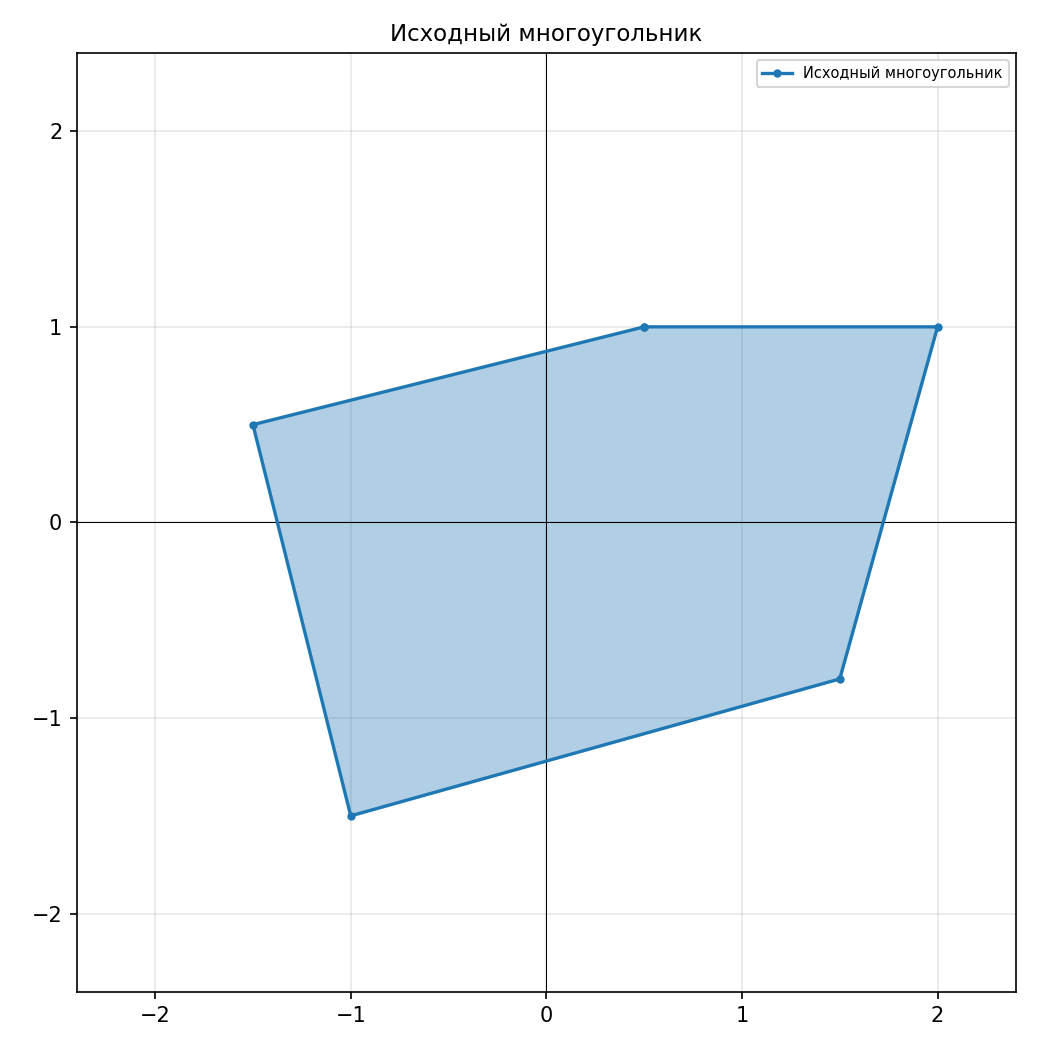
\includegraphics[width=0.55\textwidth]{../graphics/p0_polygon.png}
        \caption{Исходный многоугольник}
        \label{fig:p0}
    \end{figure}
    На всех рисунках синий цвет --- исходный многоугольник, красный --- его образ. Пунктирные прямые --- направления вещественных собственных векторов (если они есть). Образ многоугольника получается применением матрицы ко всем вершинам. Для пунктов 9 и 10 дополнительно показаны круг единичной площади и его образ.

    \section{Задание 1. Матрицы преобразований}

    \subsection{Пункт 1. Отражение относительно $y = ax$}
    \textbf{Вывод.} Пусть прямая $y=ax$ образует с осью $x$ угол $\varphi$, $\tan\varphi=a$, $u=(\cos\varphi,\sin\varphi)^T$ --- её единичный направляющий вектор. Проекция на прямую $P=uu^T$, а отражение сохраняет составляющую вдоль $u$ и меняет знак перпендикулярной: $R = P-(I-P)=2uu^T-I$. Отсюда
    $$R=\begin{pmatrix}\cos2\varphi & \sin2\varphi\\ \sin2\varphi & -\cos2\varphi\end{pmatrix}
    =\frac{1}{1+a^2}\begin{pmatrix} 1-a^2 & 2a \\ 2a & a^2-1 \end{pmatrix}.$$
    При $a=3$:
    $$M_1 = \frac{1}{10}\begin{pmatrix} -8 & 6 \\ 6 & 8 \end{pmatrix}=\begin{pmatrix} -0.8 & 0.6 \\ 0.6 & 0.8 \end{pmatrix},\quad \det M_1 = -1,\quad M_1^2=I.$$
    \begin{figure}[H]
        \centering
        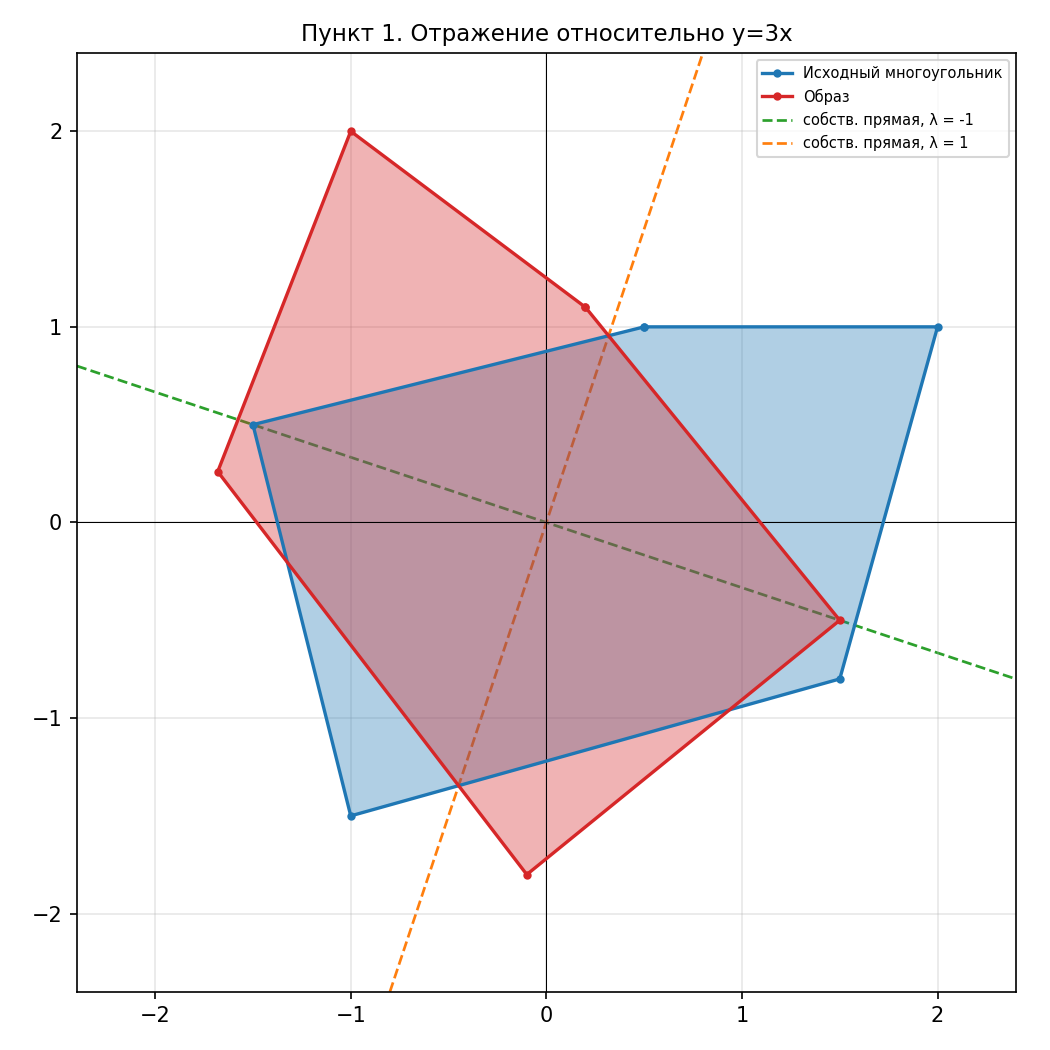
\includegraphics[width=0.65\textwidth]{../graphics/p1_reflection_y3x.png}
        \caption{Пункт 1. Отражение относительно $y=3x$}
        \label{fig:p1}
    \end{figure}

    \subsection{Пункт 2. Ортогональное отображение плоскости в прямую $y = bx$}
    \textbf{Вывод.} Это ортогональная проекция на прямую. Пусть $v=(1,b)^T/\sqrt{1+b^2}$ --- единичный направляющий вектор. Проекция точки $w$ равна $(v^Tw)v$, то есть $P = vv^T$:
    $$P = \frac{1}{1+b^2}\begin{pmatrix} 1 & b \\ b & b^2 \end{pmatrix}.$$
    Ранг равен 1, $\det P=0$, $P^2=P$, $P=P^T$. При $b=4$:
    $$M_2 = \frac{1}{17}\begin{pmatrix} 1 & 4 \\ 4 & 16 \end{pmatrix},\quad \det M_2 = 0.$$
    \begin{figure}[H]
        \centering
        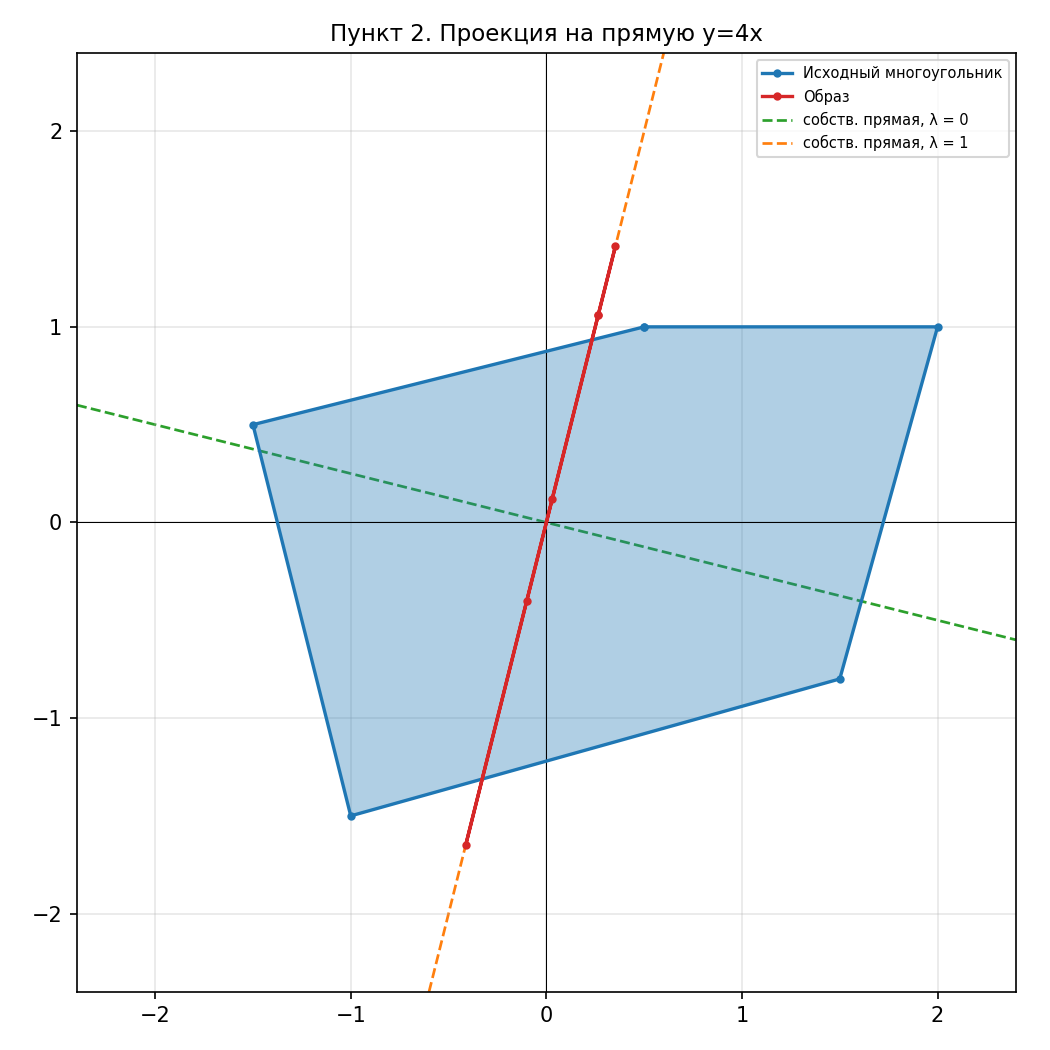
\includegraphics[width=0.65\textwidth]{../graphics/p2_projection_y4x.png}
        \caption{Пункт 2. Проекция на прямую $y=4x$}
        \label{fig:p2}
    \end{figure}

    \subsection{Пункт 3. Поворот на $10c$ градусов против часовой стрелки}
    Поворот на угол $\theta$: $R(\theta)=\begin{pmatrix}\cos\theta&-\sin\theta\\ \sin\theta&\cos\theta\end{pmatrix}$ (образы базисных векторов $(\cos\theta,\sin\theta)^T$ и $(-\sin\theta,\cos\theta)^T$ --- столбцы матрицы). При $\theta=10c=20^\circ$:
    $$M_3 = \begin{pmatrix} \cos 20^\circ & -\sin 20^\circ \\ \sin 20^\circ & \cos 20^\circ \end{pmatrix} \approx \begin{pmatrix} 0.9397 & -0.3420 \\ 0.3420 & 0.9397 \end{pmatrix},\quad \det M_3 = 1.$$
    \begin{figure}[H]
        \centering
        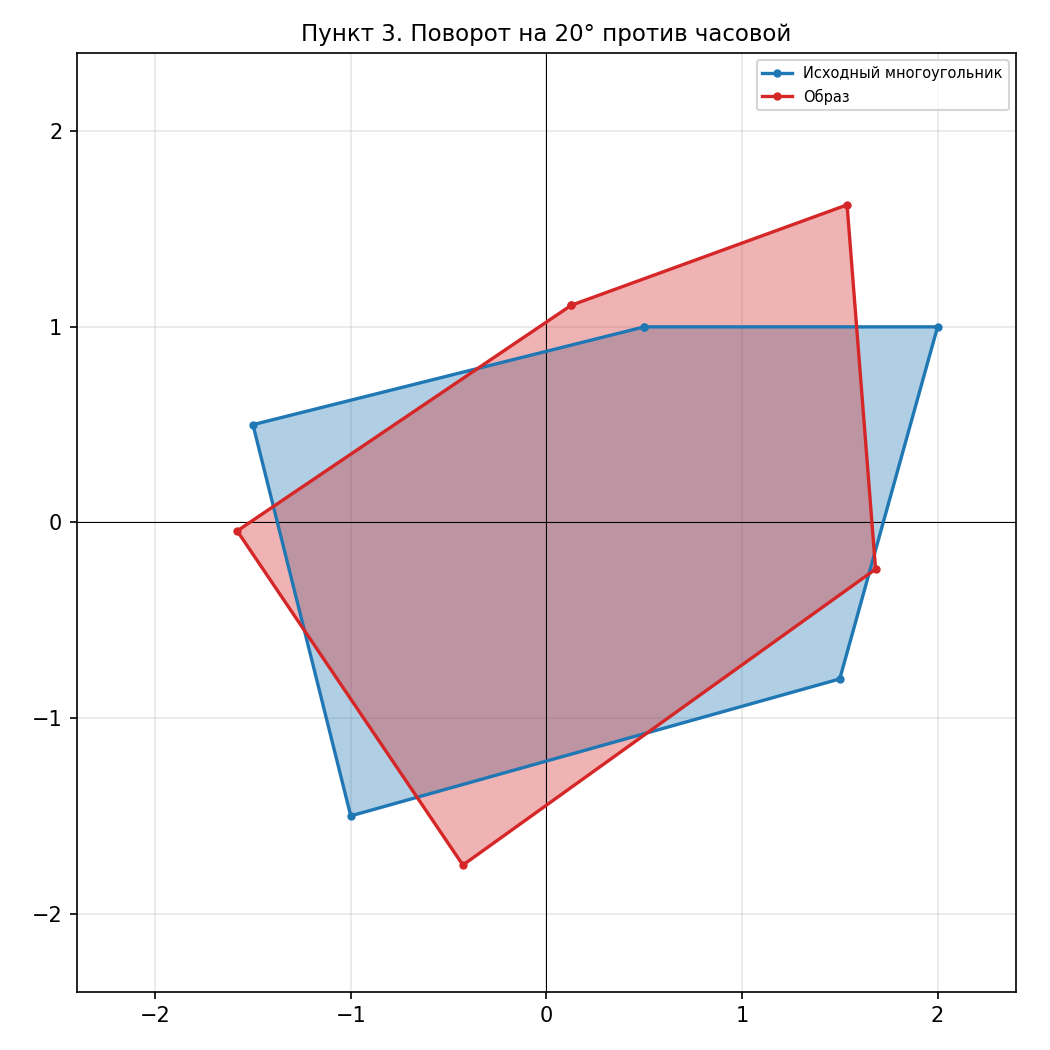
\includegraphics[width=0.65\textwidth]{../graphics/p3_rotation_20deg.png}
        \caption{Пункт 3. Поворот на $20^\circ$}
        \label{fig:p3}
    \end{figure}

    \subsection{Пункт 4. Центральная симметрия}
    Точка $(x,y)$ переходит в $(-x,-y)$, поэтому матрица равна $-I$ (это же поворот на $180^\circ$). Класс решений единственный:
    $$M_4=-I=\begin{pmatrix} -1 & 0 \\ 0 & -1 \end{pmatrix},\quad \det M_4 = 1.$$
    \begin{figure}[H]
        \centering
        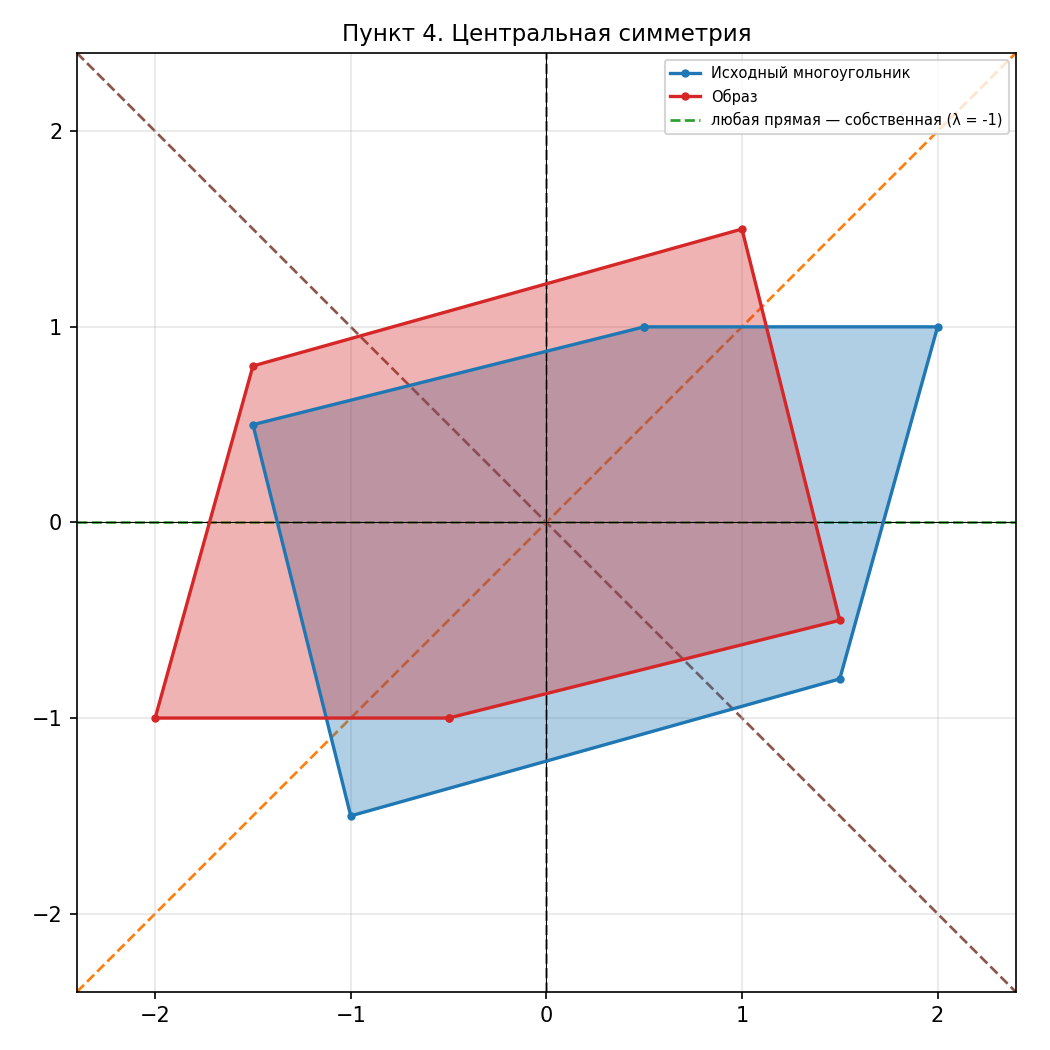
\includegraphics[width=0.65\textwidth]{../graphics/p4_central_symmetry.png}
        \caption{Пункт 4. Центральная симметрия (показаны несколько собственных прямых)}
        \label{fig:p4}
    \end{figure}

    \subsection{Пункт 5. Отражение относительно $y=ax$, затем поворот на $10d$ градусов по часовой}
    \textbf{Вывод.} При композиции матрица первого применяемого отображения стоит справа: $M_5=R(-10d^\circ)M_1=R(-50^\circ)M_1$, где $R(-50^\circ)=\begin{pmatrix}\cos50^\circ&\sin50^\circ\\ -\sin50^\circ&\cos50^\circ\end{pmatrix}$. Результат --- снова отражение: если $\varphi=\arctan3\approx71.57^\circ$, то отражение относительно прямой под углом $\varphi$, повёрнутое на угол $\alpha$, есть отражение относительно прямой под углом $\varphi+\alpha/2$. Здесь $\alpha=-50^\circ$, поэтому ось отражения лежит под углом $\varphi-25^\circ\approx46.57^\circ$:
    $$M_5=R(-50^\circ)M_1\approx\begin{pmatrix}-0.0546&0.9985\\0.9985&0.0546\end{pmatrix},\quad \det M_5=-1,\quad M_5=M_5^T,\ M_5^2=I.$$
    \begin{figure}[H]
        \centering
        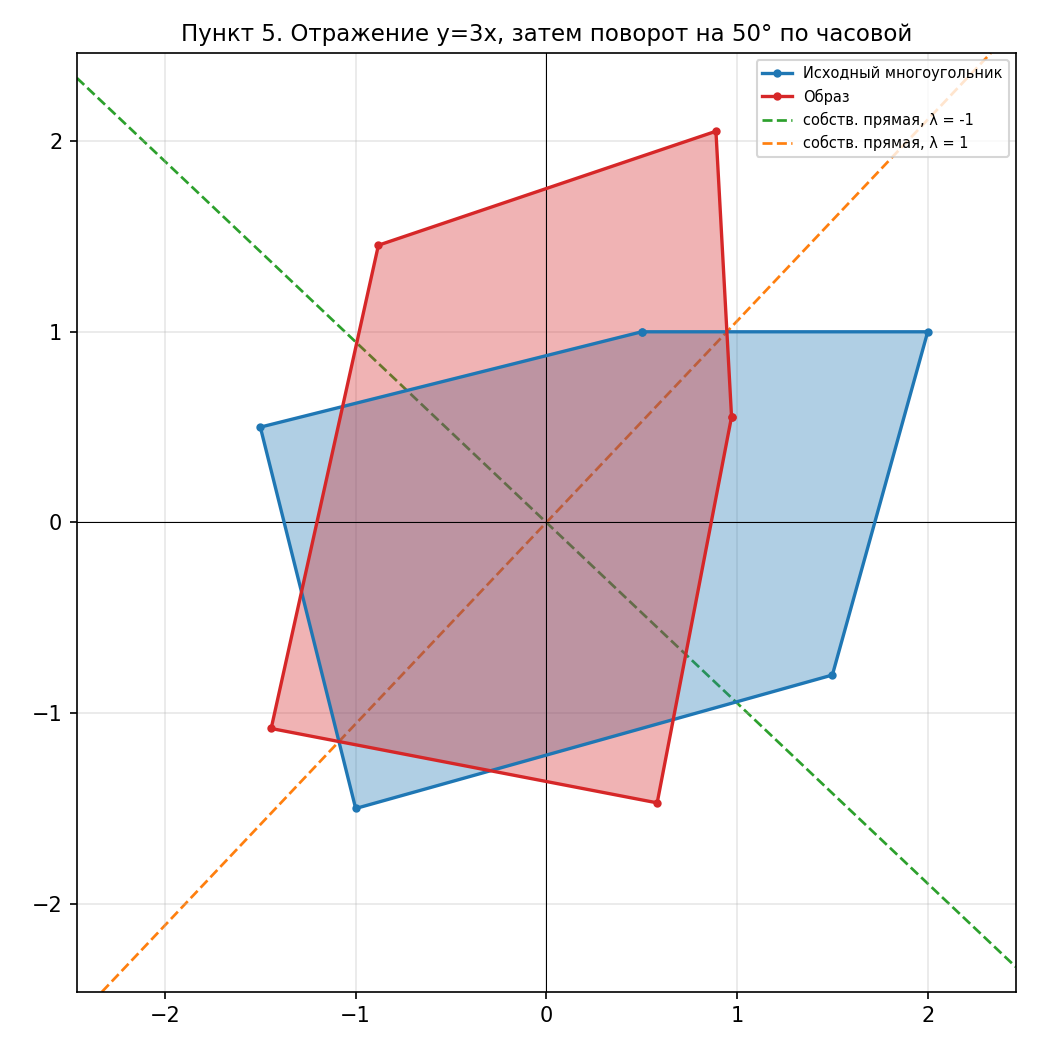
\includegraphics[width=0.65\textwidth]{../graphics/p5_reflect_then_rotate_50cw.png}
        \caption{Пункт 5. Отражение относительно $y=3x$, затем поворот на $50^\circ$ по часовой}
        \label{fig:p5}
    \end{figure}

    \subsection{Пункт 6. $y=0 \to y=ax$, $x=0 \to y=bx$}
    \textbf{Вывод.} Достаточно, чтобы $M e_1\parallel(1,a)^T$ и $Me_2\parallel(1,b)^T$, то есть $Me_1=\alpha(1,a)^T$, $Me_2=\beta(1,b)^T$ при $\alpha,\beta\neq0$. Общий класс:
    $$M=\begin{pmatrix}\alpha&\beta\\ a\alpha&b\beta\end{pmatrix}=\begin{pmatrix}1&1\\a&b\end{pmatrix}\begin{pmatrix}\alpha&0\\0&\beta\end{pmatrix}.$$
    Берём $\alpha=1$, $\beta=2$ (чтобы матрица была не слишком простой):
    $$M_6 = \begin{pmatrix} 1 & 2 \\ 3 & 8 \end{pmatrix},\quad \det M_6 = 2.$$
    Проверка: $M_6(1,0)^T=(1,3)^T$ лежит на $y=3x$, $M_6(0,1)^T=(2,8)^T$ лежит на $y=4x$. Так как $M_6$ невырождена, образы осей --- именно эти прямые целиком.
    \begin{figure}[H]
        \centering
        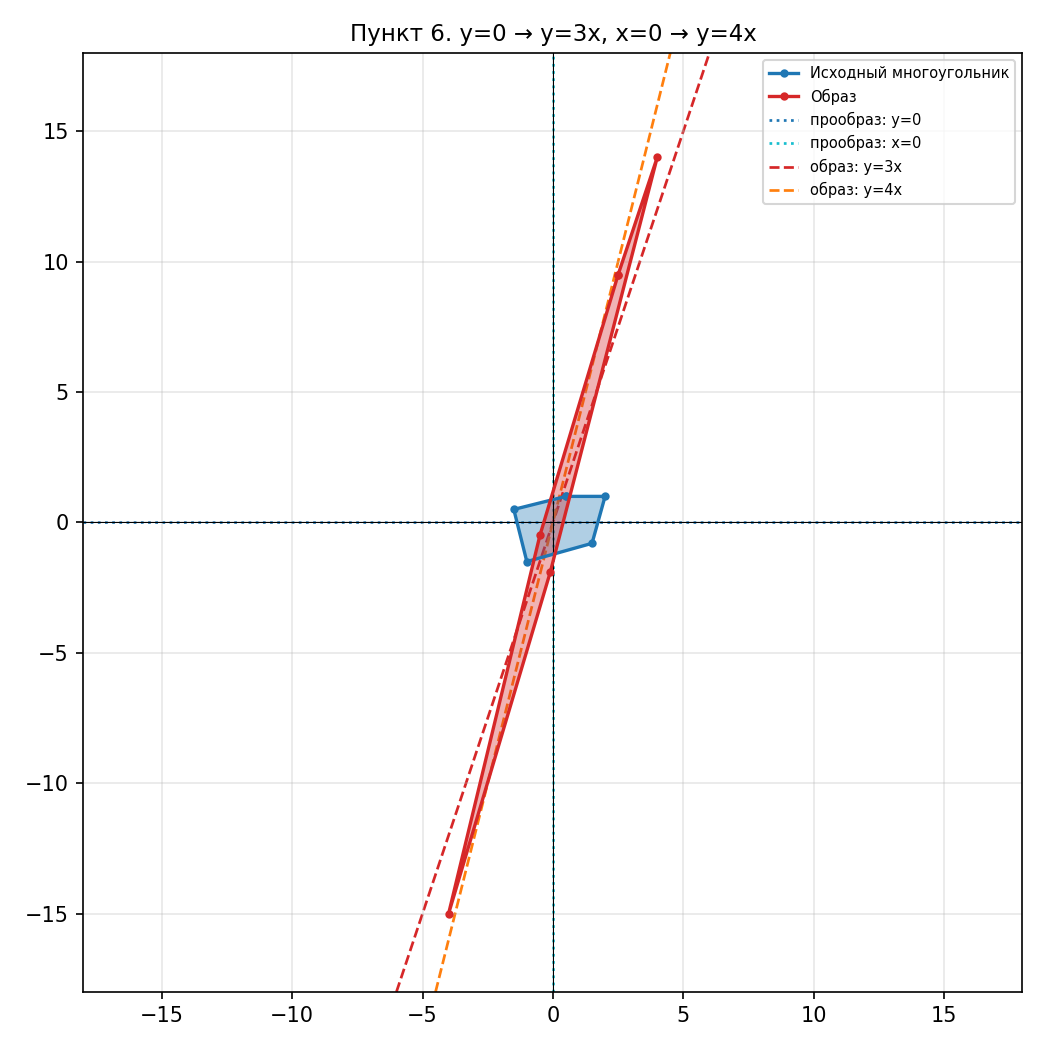
\includegraphics[width=0.65\textwidth]{../graphics/p6_map_y0_to_y3x.png}
        \caption{Пункт 6. Прямая $y=0$ переходит в $y=3x$, прямая $x=0$ --- в $y=4x$}
        \label{fig:p6}
    \end{figure}

    \subsection{Пункт 7. $y=ax \to y=0$, $y=bx \to x=0$}
    \textbf{Вывод.} Пусть $p_1=(1,a)^T$, $p_2=(1,b)^T$, $Q=(p_1\,|\,p_2)$. Требуется $Mp_1=\alpha e_1$, $Mp_2=\beta e_2$, то есть $MQ=\mathrm{diag}(\alpha,\beta)$. Общий класс:
    $$M=\begin{pmatrix}\alpha&0\\0&\beta\end{pmatrix}Q^{-1},\quad Q^{-1}=\frac{1}{b-a}\begin{pmatrix}b&-1\\-a&1\end{pmatrix}.$$
    При $a=3$, $b=4$, $\alpha=\beta=1$ ($b-a=1$):
    $$M_7 = \begin{pmatrix} 4 & -1 \\ -3 & 1 \end{pmatrix},\quad \det M_7 = 1.$$
    Проверка: $M_7(1,3)^T=(1,0)^T$, $M_7(1,4)^T=(0,1)^T$.
    \begin{figure}[H]
        \centering
        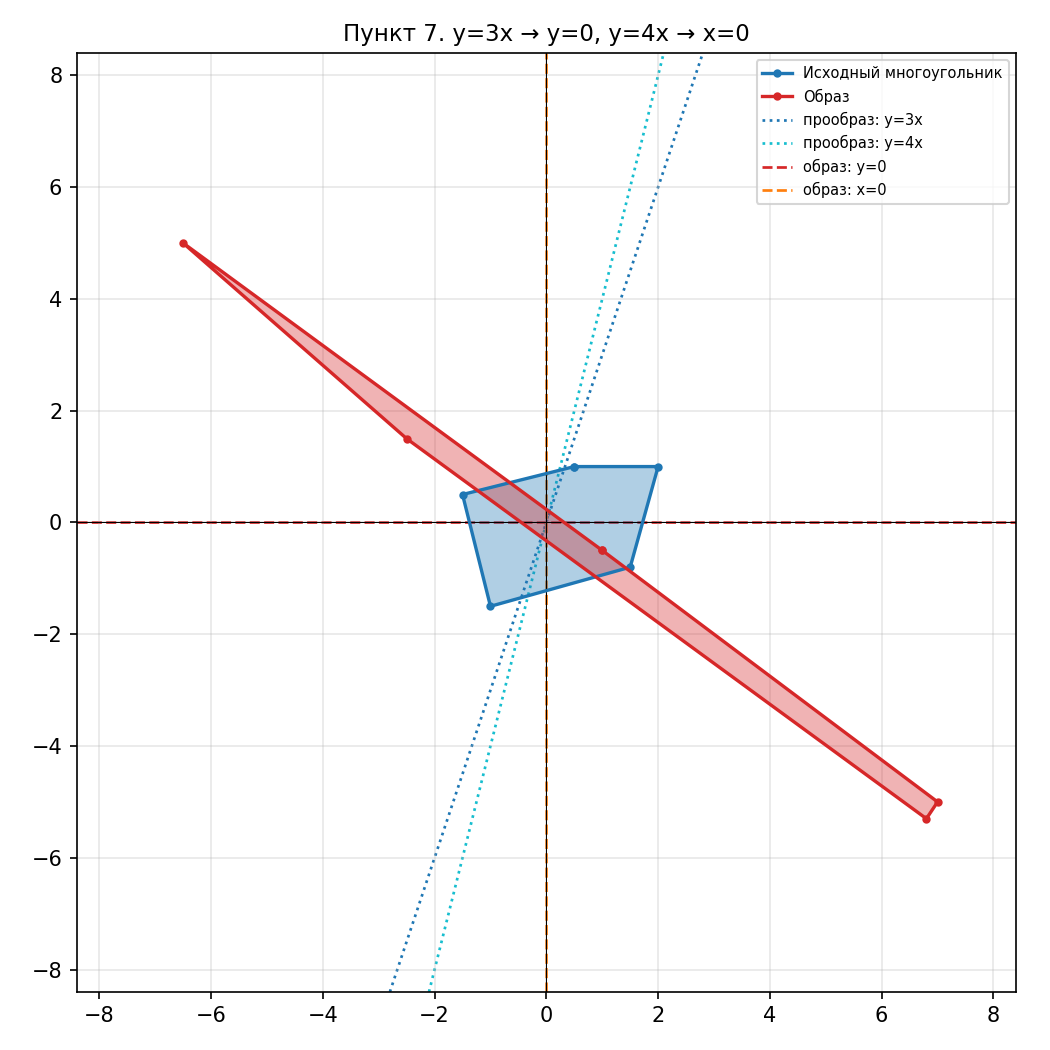
\includegraphics[width=0.65\textwidth]{../graphics/p7_map_y3x_to_y0.png}
        \caption{Пункт 7. Прямая $y=3x$ переходит в $y=0$, прямая $y=4x$ --- в $x=0$}
        \label{fig:p7}
    \end{figure}

    \subsection{Пункт 8. Меняет местами прямые $y=ax$ и $y=bx$}
    \textbf{Вывод.} Нужно $Mp_1=\alpha p_2$, $Mp_2=\beta p_1$, то есть $MQ=Q\begin{pmatrix}0&\alpha\\ \beta&0\end{pmatrix}$. Общий класс:
    $$M=Q\begin{pmatrix}0&\alpha\\ \beta&0\end{pmatrix}Q^{-1},\quad Q=\begin{pmatrix}1&1\\a&b\end{pmatrix}.$$
    При $\alpha=\beta=1$:
    $$M_8 = \begin{pmatrix} 1 & 0 \\ 7 & -1 \end{pmatrix},\quad \det M_8 = -1,\quad M_8^2=I.$$
    Проверка: $M_8(1,3)^T=(1,4)^T$, $M_8(1,4)^T=(1,3)^T$. Эта матрица не симметрична (отражение вдоль неперпендикулярных направлений).
    \begin{figure}[H]
        \centering
        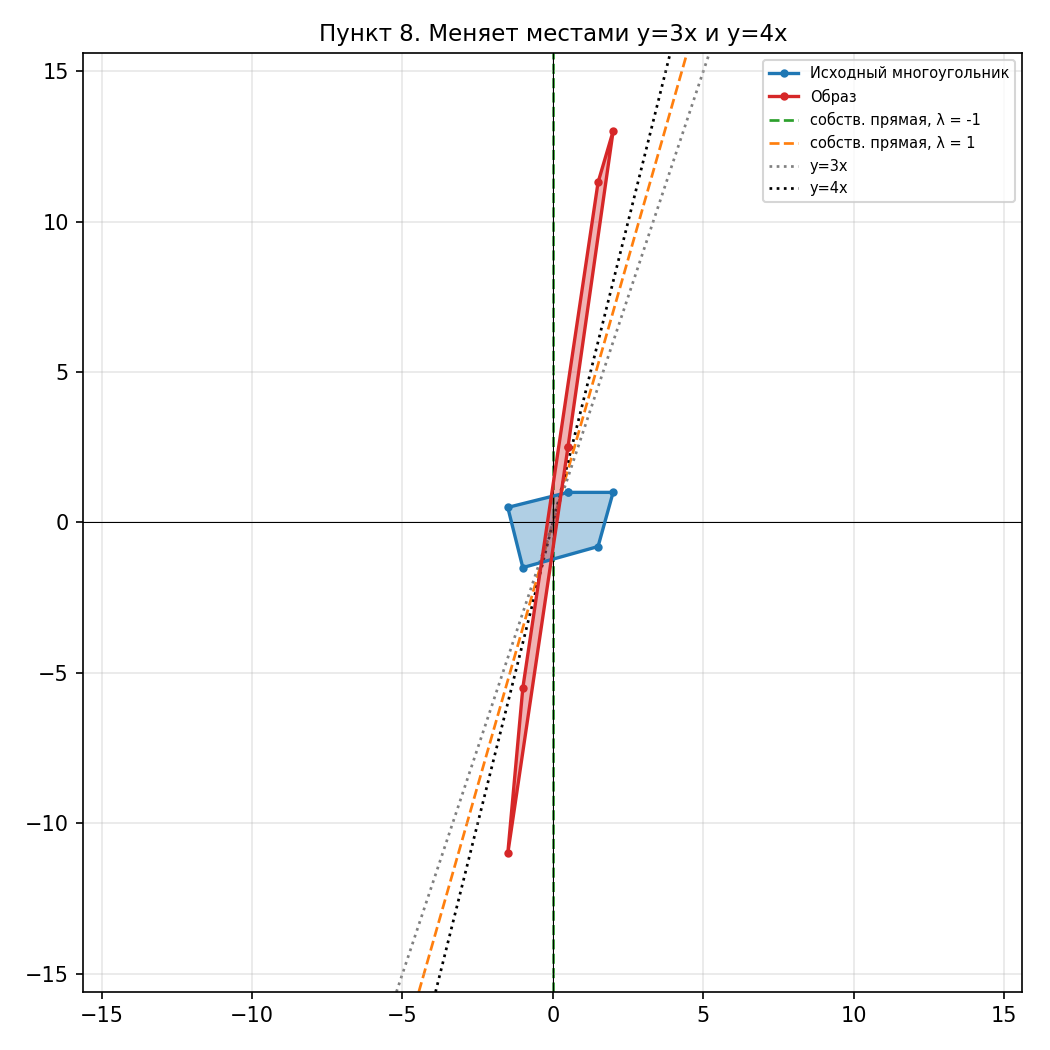
\includegraphics[width=0.65\textwidth]{../graphics/p8_swap_lines.png}
        \caption{Пункт 8. Меняет местами прямые $y=3x$ и $y=4x$; пунктиром --- собственные прямые}
        \label{fig:p8}
    \end{figure}

    \subsection{Пункт 9. Недиагональная матрица: круг площади 1 $\to$ круг площади $c$}
    \textbf{Вывод.} Площадь образа равна $|\det M|$ площади прообраза, поэтому $|\det M|=c=2$. Но образ должен быть именно кругом, а не эллипсом, а это возможно только если $M^TM=kI$ (у матрицы равные сингулярные числа), то есть $M=\sqrt{k}\,Q$ с ортогональной $Q$. Из $\det M=\pm k=\pm c$ получаем $k=c$. Общий класс:
    $$M=\sqrt{c}\,Q,\quad Q\in O(2),\quad Q\neq\pm I,\ Q\ \text{недиагональна}.$$
    Берём поворот на $45^\circ$: $M=\sqrt2\,R(45^\circ)$:
    $$M_9 = \begin{pmatrix} 1 & -1 \\ 1 & 1 \end{pmatrix},\quad M_9^TM_9=2I,\quad \det M_9 = 2.$$
    Образ круга радиуса $r=1/\sqrt\pi$ --- круг радиуса $\sqrt2\,r$ и площади $2$. (Матрица $\begin{pmatrix}2&1\\0&1\end{pmatrix}$ тоже имеет определитель 2, но переводит круг в эллипс, поэтому не подходит.)
    \begin{figure}[H]
        \centering
        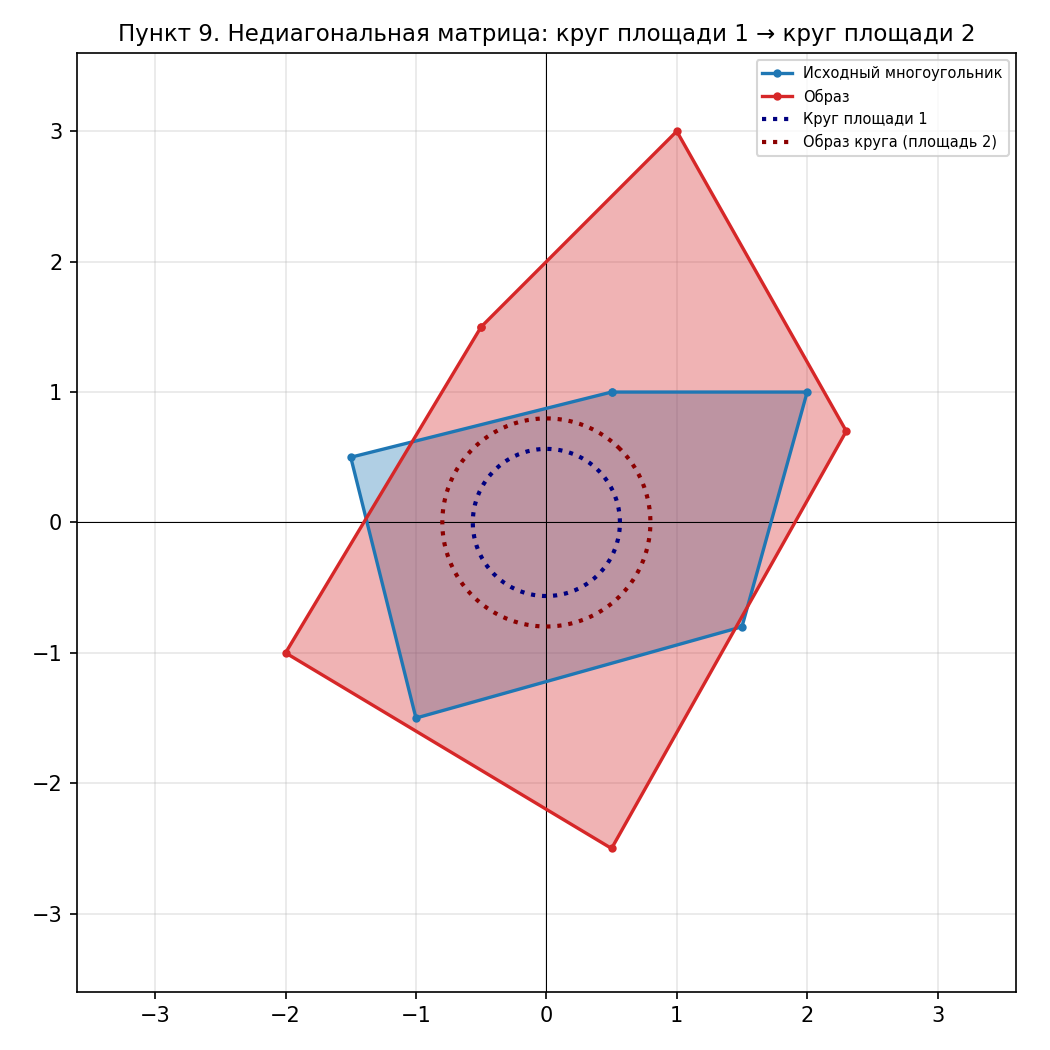
\includegraphics[width=0.65\textwidth]{../graphics/p9_nondiagonal_circle_2.png}
        \caption{Пункт 9. $\det=2$, круг площади 1 переходит в круг площади 2}
        \label{fig:p9}
    \end{figure}

    \subsection{Пункт 10. Недиагональная матрица: круг площади 1 $\to$ некруг площади $d$}
    \textbf{Вывод.} Нужно $|\det M|=d=5$ и неравные сингулярные числа. Удобно взять симметричную матрицу $M=QDQ^T$ с $D=\mathrm{diag}(1,d)$ и поворотом $Q=R(30^\circ)$: собственные числа $1$ и $5$ различны, значит образ круга --- эллипс с полуосями $r$ и $5r$ ($r=1/\sqrt\pi$), площадь $\pi\cdot r\cdot5r=5$. Недиагональность обеспечивает $Q\neq I$:
    $$M_{10} = R(30^\circ)\begin{pmatrix} 1 & 0 \\ 0 & 5 \end{pmatrix}R(30^\circ)^T=\begin{pmatrix}2&-\sqrt3\\-\sqrt3&4\end{pmatrix},\quad \det M_{10} = 5.$$
    Собственные векторы: $(\cos30^\circ,\sin30^\circ)^T$ при $\lambda=1$ и $(-\sin30^\circ,\cos30^\circ)^T$ при $\lambda=5$.
    \begin{figure}[H]
        \centering
        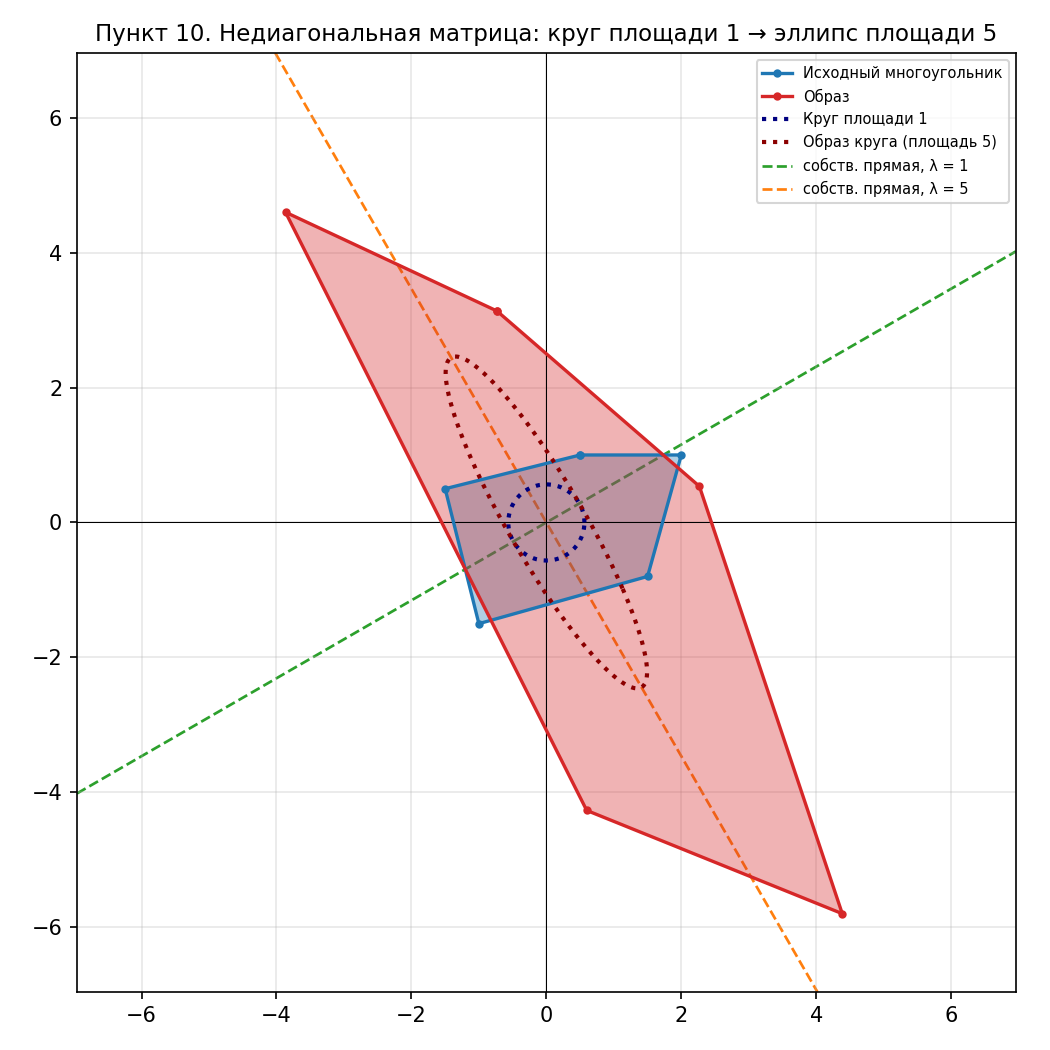
\includegraphics[width=0.65\textwidth]{../graphics/p10_nondiagonal_noncircle_5.png}
        \caption{Пункт 10. $\det=5$, круг площади 1 переходит в эллипс площади 5}
        \label{fig:p10}
    \end{figure}

    \subsection{Пункт 11. Перпендикулярные собственные векторы, не лежащие на $y=0$ и $y=x$}
    \textbf{Вывод.} Матрица с вещественными собственными числами и ортогональными собственными векторами --- это в точности симметричная матрица $M=Q\,\mathrm{diag}(\lambda_1,\lambda_2)Q^T$, $Q\in O(2)$. Нужно, чтобы столбцы $Q$ не были направлены вдоль $y=0$ и $y=x$. Возьмём
    $$M_{11} = \begin{pmatrix} 3 & 1 \\ 1 & 1 \end{pmatrix}.$$
    Характеристический многочлен $\lambda^2-4\lambda+2=0$, $\lambda=2\pm\sqrt2$. Из $(3-\lambda)x+y=0$ получаем $y=(\lambda-3)x$:
    $$\lambda_1=2+\sqrt2:\ v_1=(1,\sqrt2-1)^T,\qquad \lambda_2=2-\sqrt2:\ v_2=(1,-1-\sqrt2)^T.$$
    Перпендикулярность: $v_1^Tv_2=1+(\sqrt2-1)(-1-\sqrt2)=1-(\sqrt2-1)(\sqrt2+1)=1-1=0$. Угловые коэффициенты $\sqrt2-1\approx0.414$ и $-1-\sqrt2\approx-2.414$ не равны $0$ и $1$, значит прямые не совпадают с $y=0$ и $y=x$.
    \begin{figure}[H]
        \centering
        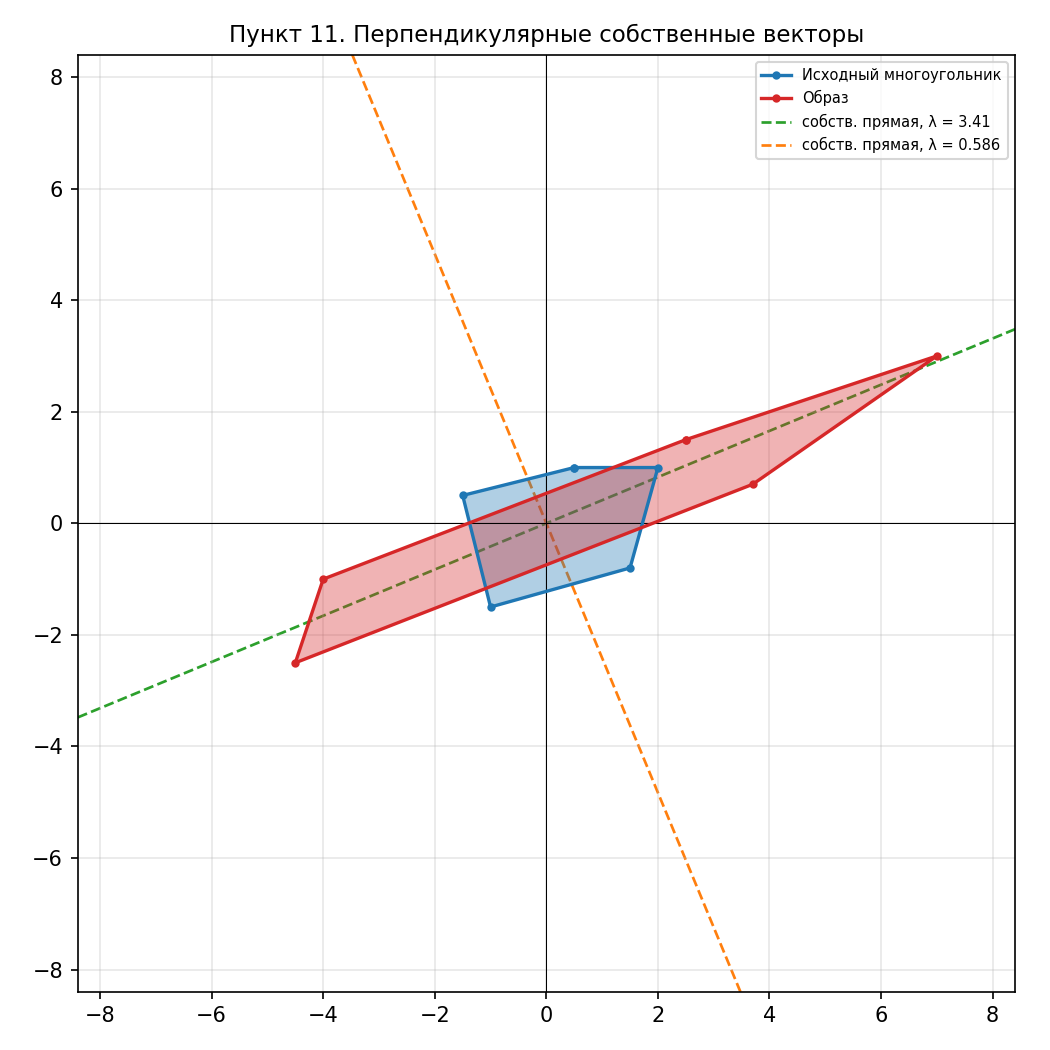
\includegraphics[width=0.65\textwidth]{../graphics/p11_perpendicular_eigenvectors.png}
        \caption{Пункт 11. Симметричная матрица с перпендикулярными собственными векторами}
        \label{fig:p11}
    \end{figure}

    \subsection{Пункт 12. Нет двух неколлинеарных собственных векторов}
    \textbf{Вывод.} Матрица $2\times2$ не имеет двух неколлинеарных собственных векторов тогда и только тогда, когда она недиагонализуема, то есть имеет кратное собственное число $\lambda$ и не равна $\lambda I$. Общий класс: $M=\lambda I+N$, где $N\neq0$, $N^2=0$ (например, $P\begin{pmatrix}\lambda&1\\0&\lambda\end{pmatrix}P^{-1}$). Берём жорданову клетку
    $$M_{12} = \begin{pmatrix} 2 & 1 \\ 0 & 2 \end{pmatrix}.$$
    $(\lambda-2)^2=0$, алгебраическая кратность равна 2. Из $(M_{12}-2I)v=\begin{pmatrix}0&1\\0&0\end{pmatrix}v=0$ получаем $v\parallel(1,0)^T$, то есть геометрическая кратность равна 1. Обобщённый собственный вектор: $(M_{12}-2I)w=v$, $w=(0,1)^T$.
    \begin{figure}[H]
        \centering
        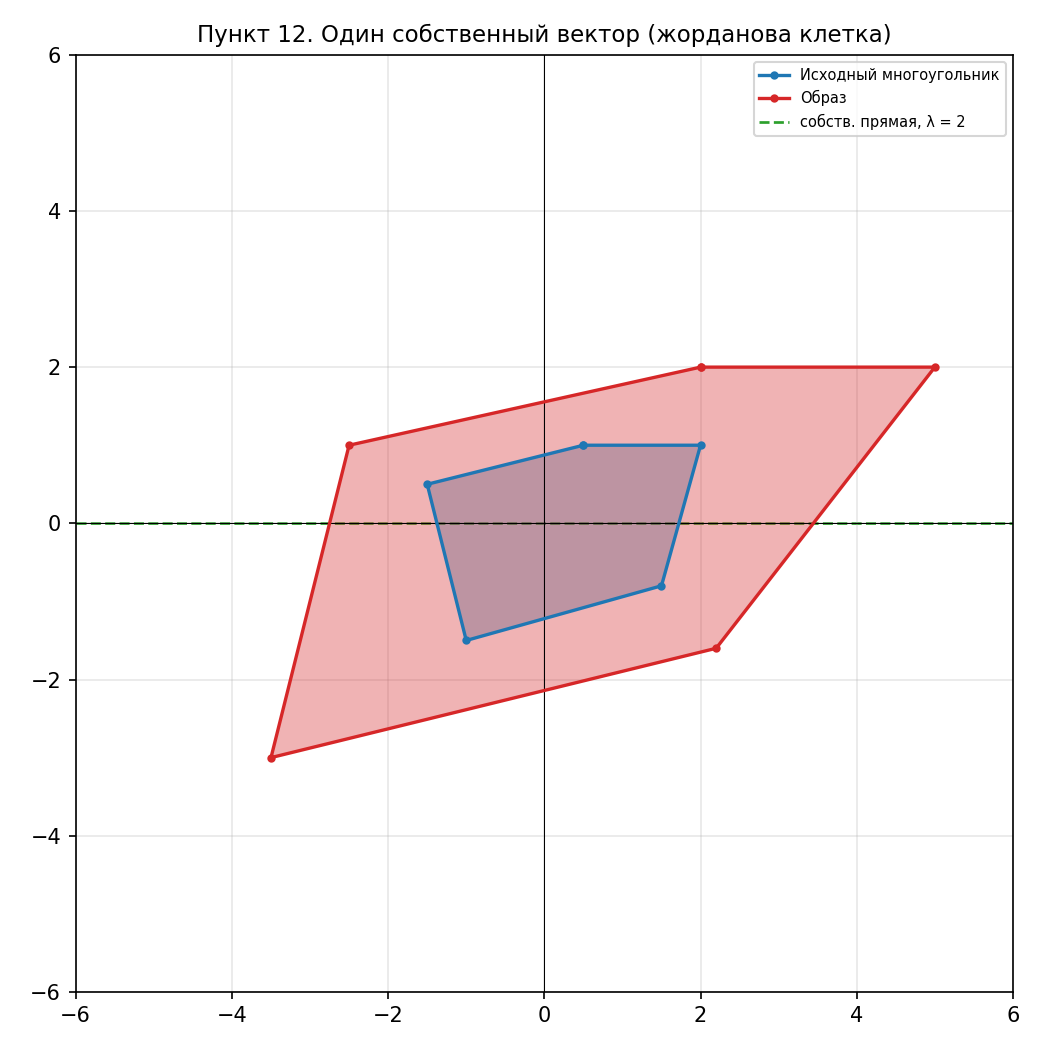
\includegraphics[width=0.65\textwidth]{../graphics/p12_no_two_eigenvectors.png}
        \caption{Пункт 12. Жорданова клетка --- единственная собственная прямая}
        \label{fig:p12}
    \end{figure}

    \subsection{Пункт 13. Нет ни одного вещественного собственного вектора}
    \textbf{Вывод.} Вещественный собственный вектор существует тогда и только тогда, когда у характеристического многочлена $\lambda^2-\tr M\,\lambda+\det M$ есть вещественный корень. Поэтому условие отсутствия: $(\tr M)^2<4\det M$. Общий класс: $M=P\begin{pmatrix}\alpha&-\beta\\ \beta&\alpha\end{pmatrix}P^{-1}$, $\beta\neq0$. Возьмём поворот на $90^\circ$:
    $$M_{13} = \begin{pmatrix} 0 & -1 \\ 1 & 0 \end{pmatrix},\quad \tr=0,\ \det=1,\ 0<4.$$
    $\lambda^2+1=0$, $\lambda=\pm i$, комплексные собственные векторы $(1,\mp i)^T$. На плоскости $\mathbb R^2$ ни одна прямая не переходит в себя (кроме как при повороте на $0^\circ$ и $180^\circ$).
    \begin{figure}[H]
        \centering
        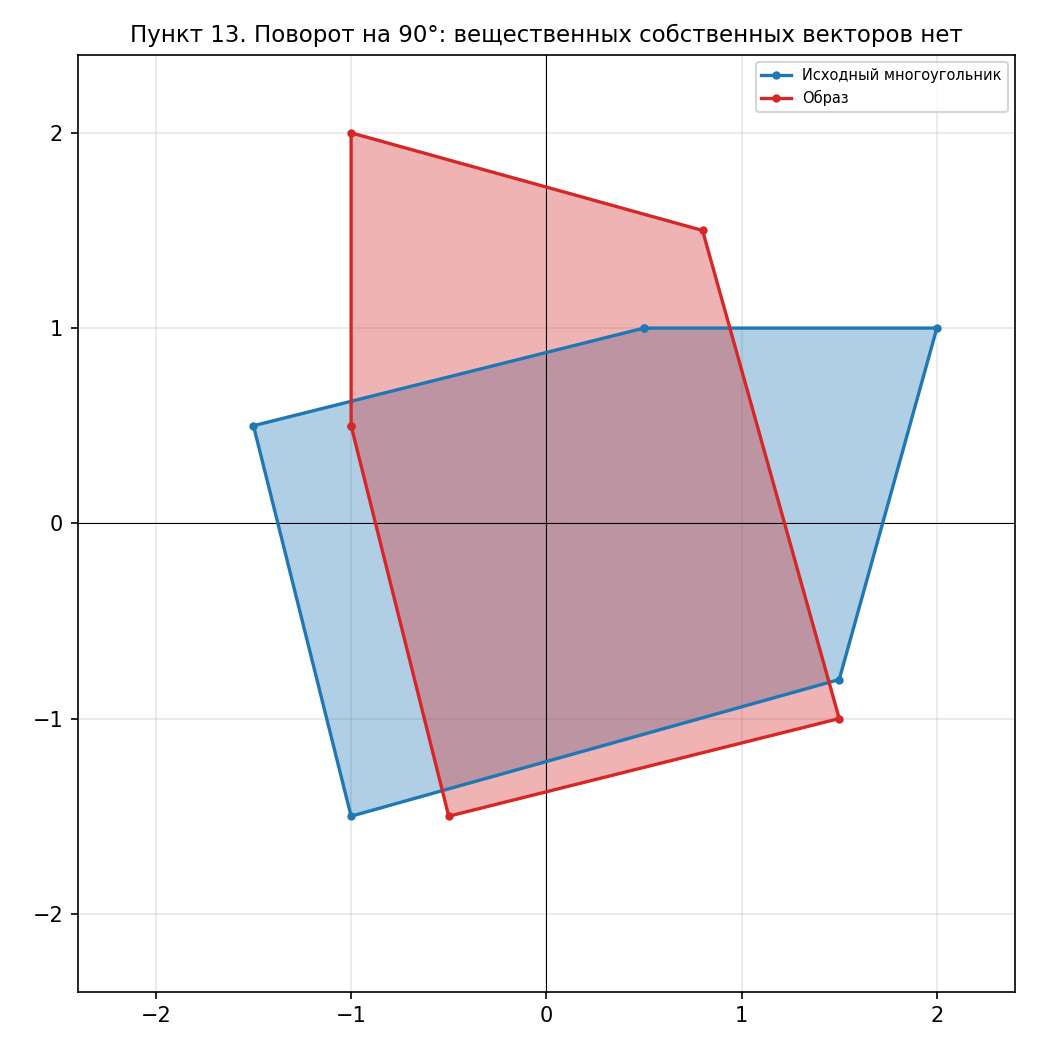
\includegraphics[width=0.65\textwidth]{../graphics/p13_no_real_eigenvectors.png}
        \caption{Пункт 13. Поворот на $90^\circ$: вещественных собственных прямых нет}
        \label{fig:p13}
    \end{figure}

    \subsection{Пункт 14. Любой ненулевой вектор является собственным}
    \textbf{Вывод.} Если $Me_1=\lambda_1e_1$, $Me_2=\lambda_2e_2$ и $M(e_1+e_2)=\mu(e_1+e_2)$, то $\lambda_1=\mu=\lambda_2$. Поэтому условие выполняется тогда и только тогда, когда $M=\lambda I$. Берём $\lambda=2$:
    $$M_{14} = 2I = \begin{pmatrix} 2 & 0 \\ 0 & 2 \end{pmatrix},\quad \det M_{14}=4.$$
    \begin{figure}[H]
        \centering
        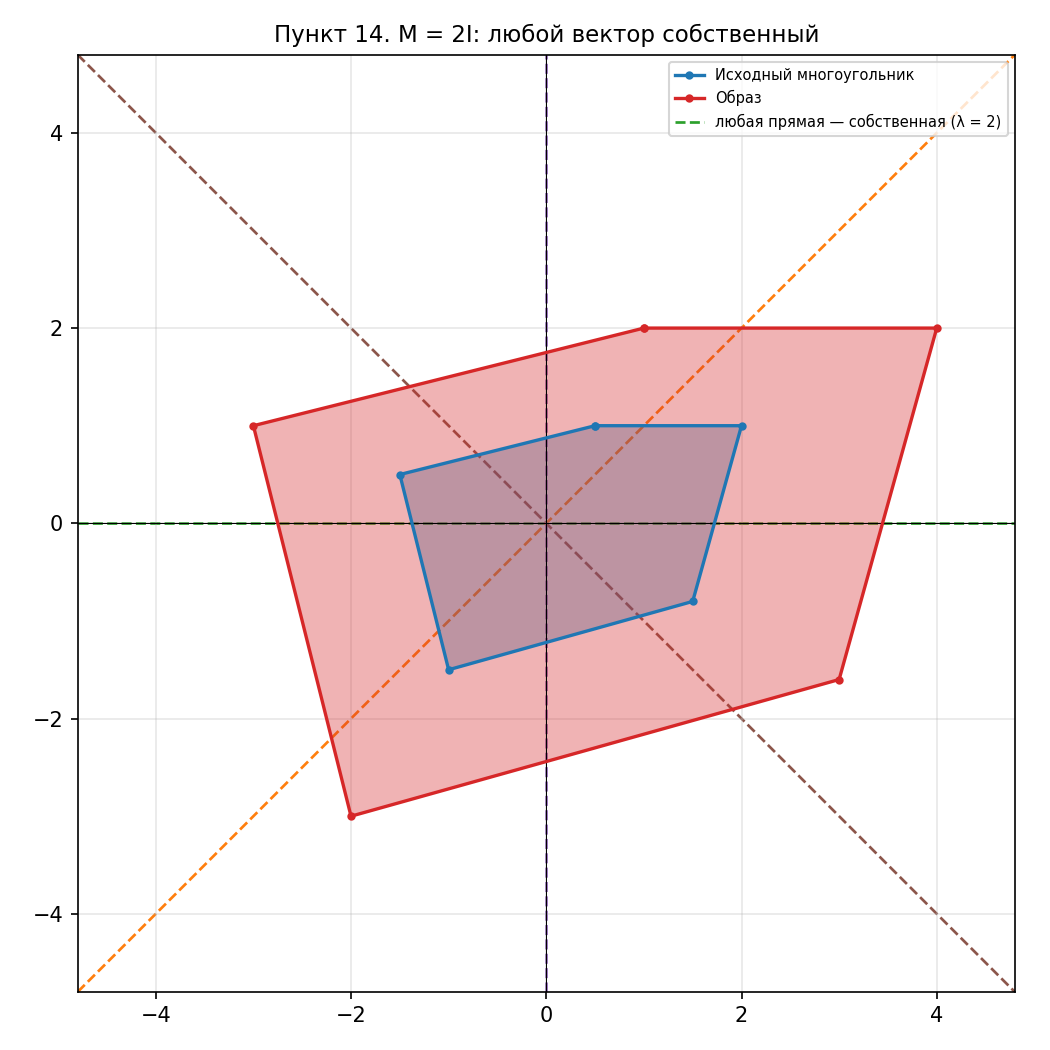
\includegraphics[width=0.65\textwidth]{../graphics/p14_any_vector_eigen.png}
        \caption{Пункт 14. $M=2I$: любая прямая через начало --- собственная}
        \label{fig:p14}
    \end{figure}

    \subsection{Пункт 15. $AB\neq BA$}
    \textbf{Вывод.} Берём $A=M_3=R(20^\circ)$ и $B=M_1$ (отражение). Поскольку $R(\theta)\,\mathrm{Ref}(\varphi)=\mathrm{Ref}(\varphi+\theta/2)$, а $\mathrm{Ref}(\varphi)\,R(\theta)=\mathrm{Ref}(\varphi-\theta/2)$, матрицы $AB$ и $BA$ --- отражения относительно разных прямых (под углами $\varphi\pm10^\circ$, где $\varphi=\arctan 3\approx71.57^\circ$), так что $AB\ne BA$ при любом $\theta$, не кратном $180^\circ$. Численно:
    $$AB\approx\begin{pmatrix}-0.9570&0.2902\\0.2902&0.9570\end{pmatrix},\qquad BA\approx\begin{pmatrix}-0.5465&0.8374\\0.8374&0.5465\end{pmatrix}.$$
    Порядок применения важен: $AB$ --- сначала отражение, затем поворот; $BA$ --- сначала поворот, затем отражение. На рисунке показаны исходный многоугольник, $A$, $B$, $AB$, $BA$ и наложение $AB$ на $BA$.
    \begin{figure}[H]
        \centering
        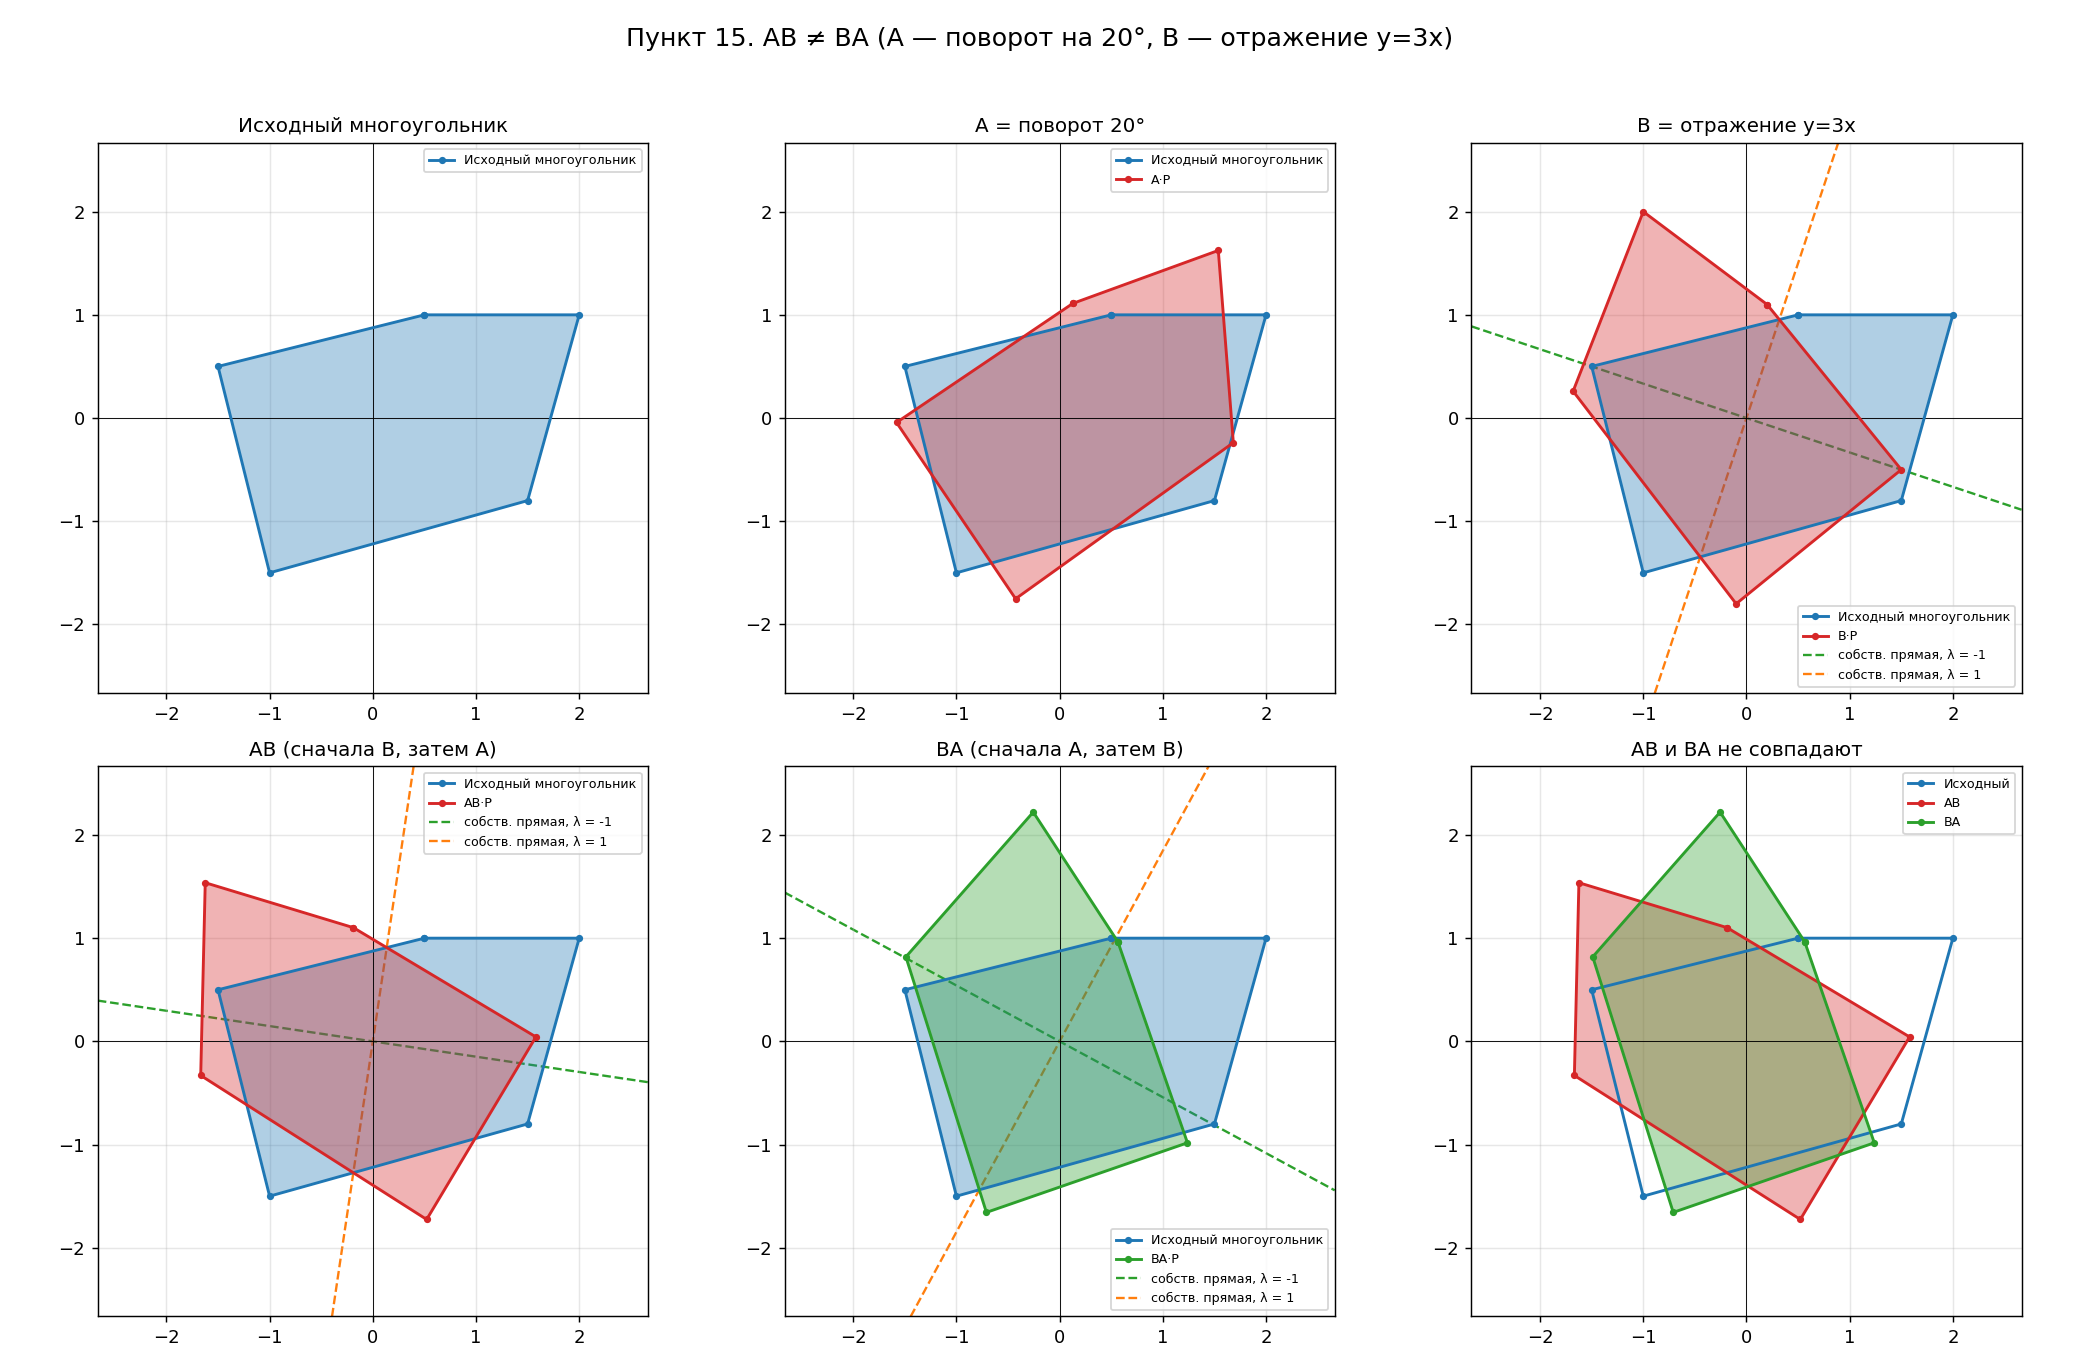
\includegraphics[width=\textwidth]{../graphics/p15_AB_BA_composition.png}
        \caption{Пункт 15. $AB\neq BA$}
        \label{fig:p15}
    \end{figure}

    \subsection{Пункт 16. $AB=BA$, максимально непохожие матрицы}
    \textbf{Вывод.} Для не скалярной матрицы $A$ размера $2\times2$ коммутирующие с ней матрицы --- это в точности $B=\alpha I+\beta A$. Значит, у $A$ и $B$ всегда общие собственные векторы, но остальные свойства можно сделать совсем разными. Берём отражение $A=M_1$ (ортогональная, инволютивная, $\det=-1$, собственные числа $\pm1$) и
    $$B=3I+5A=\begin{pmatrix}-1&3\\3&7\end{pmatrix}$$
    (не ортогональная, не инволютивная, $\det B=-16$, собственные числа $8$ и $-2$). Тогда
    $$AB=BA=3A+5I=\frac15\begin{pmatrix}13&9\\9&37\end{pmatrix},\quad\text{собственные числа }8\ \text{и}\ 2.$$
    Тривиальный вариант $B=I$ тоже коммутирует с любой матрицей, но матрицы $A$ и $I$ слишком похожи по смыслу, поэтому взята нетривиальная пара.
    \begin{figure}[H]
        \centering
        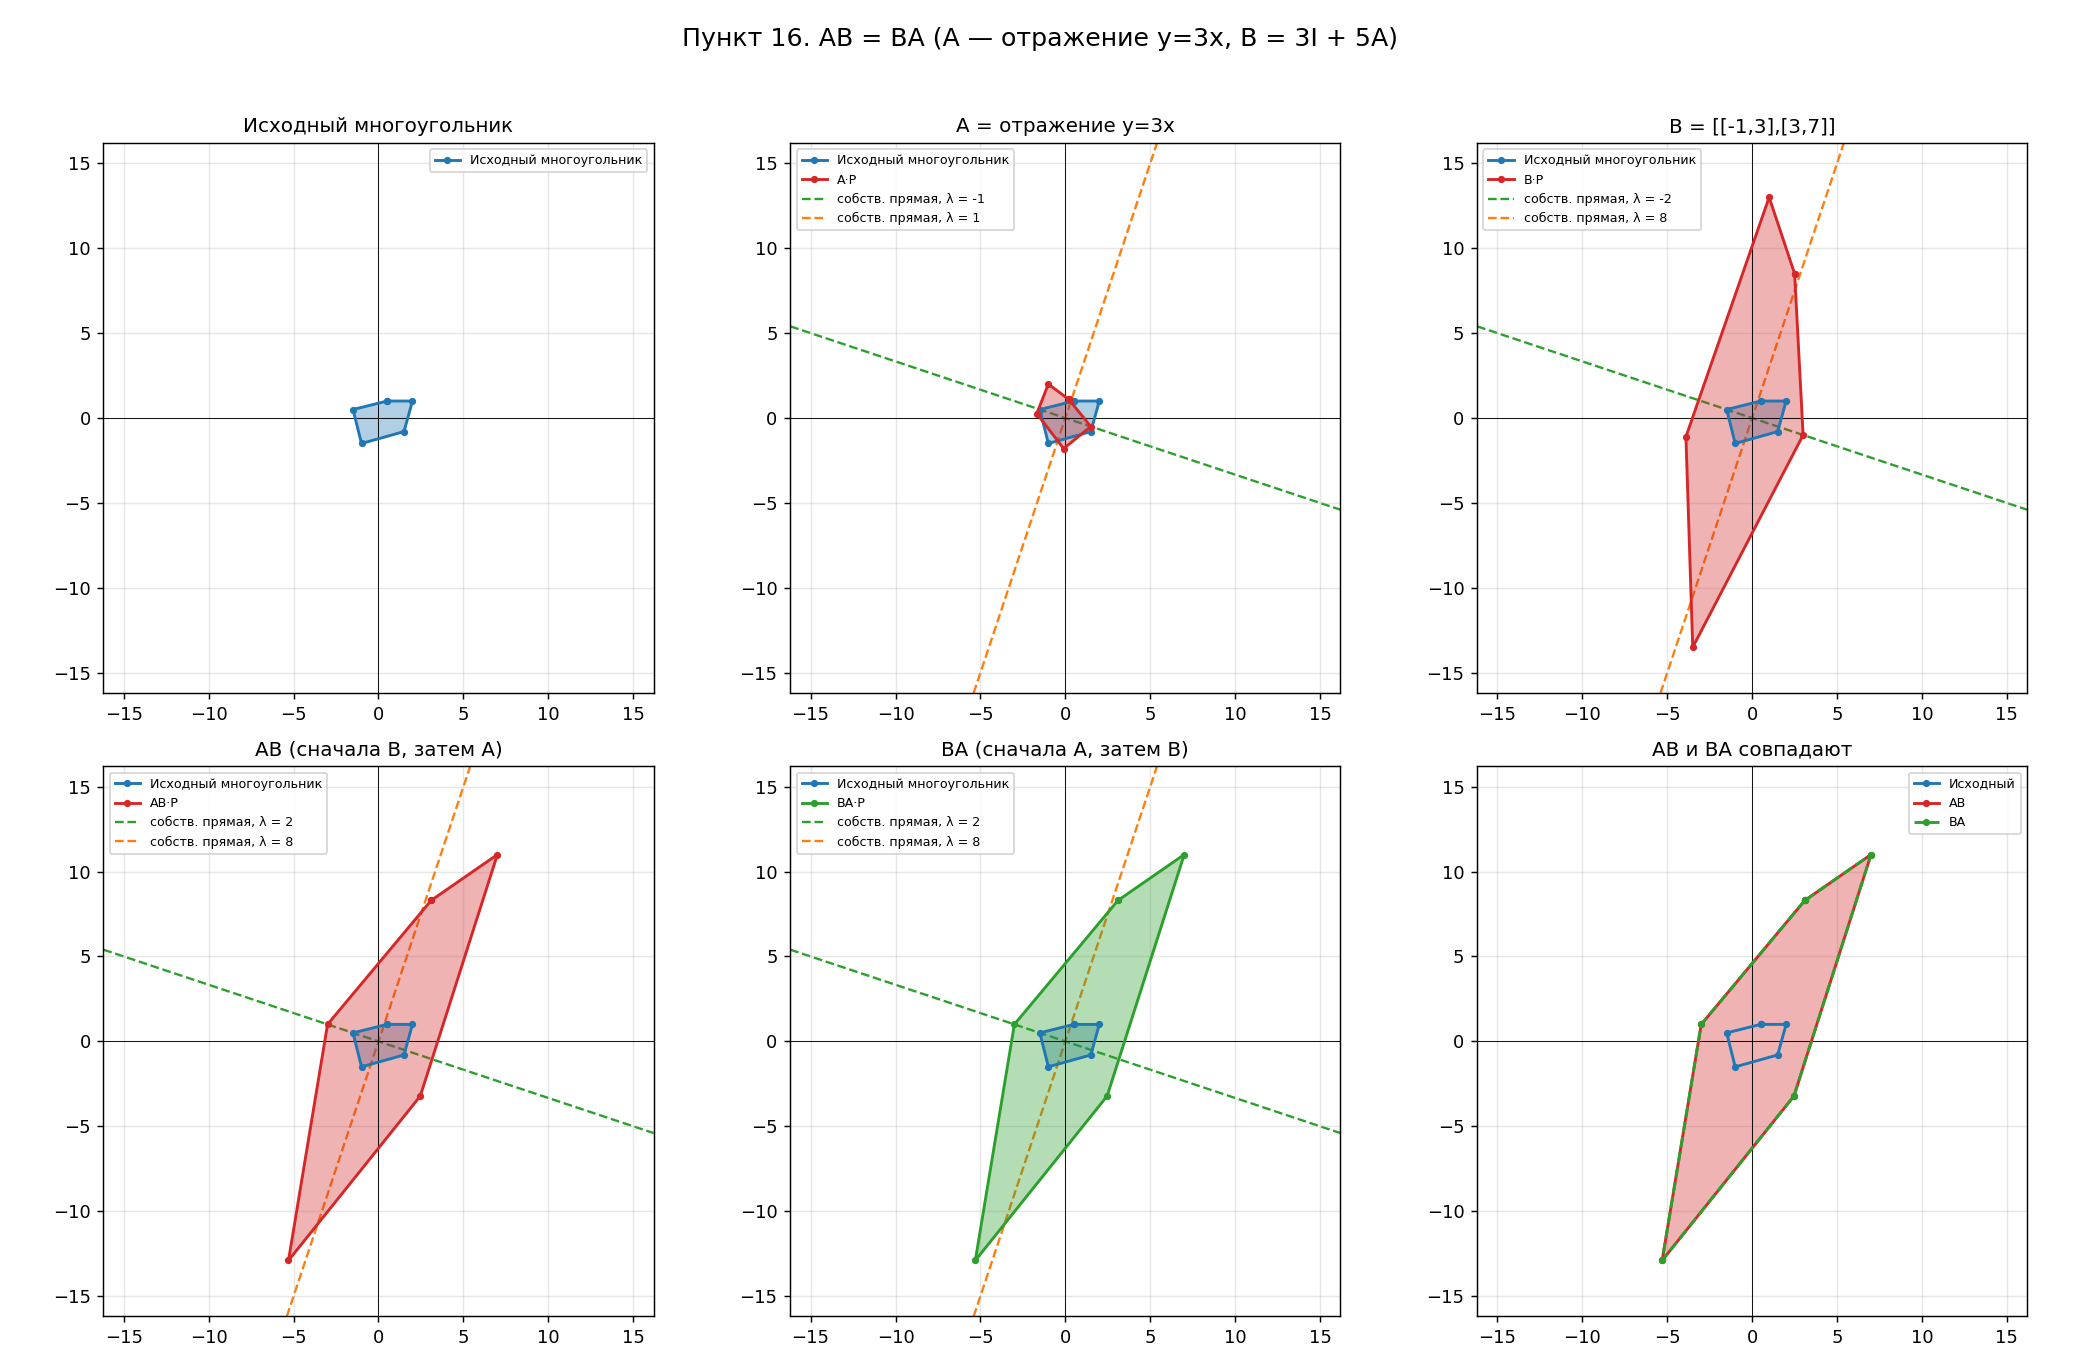
\includegraphics[width=\textwidth]{../graphics/p16_AB_eq_BA.png}
        \caption{Пункт 16. $AB=BA$}
        \label{fig:p16}
    \end{figure}

    \section{Задание 2. Анализ отображений}
    \subsection{Образ и ядро}
    \begin{itemize}
        \item[П.1] $\det M_1=-1\neq0$: $\mathrm{Im}=\mathbb R^2$, $\ker=\{0\}$.
        \item[П.2] $\rank M_2=1$: $\mathrm{Im}=\{y=4x\}=\langle(1,4)^T\rangle$, $\ker=\langle(4,-1)^T\rangle$ (проверка: $M_2(4,-1)^T=\frac1{17}(0,0)^T$). $\dim\mathrm{Im}+\dim\ker=2$.
        \item[П.13] $\det M_{13}=1\neq0$: $\mathrm{Im}=\mathbb R^2$, $\ker=\{0\}$.
        \item[П.14] $\det M_{14}=4\neq0$: $\mathrm{Im}=\mathbb R^2$, $\ker=\{0\}$.
    \end{itemize}

    \subsection{Собственные числа и векторы}
    \begin{itemize}
        \item[П.1] $\lambda=1$, $v=(1,3)^T$ (на оси отражения); $\lambda=-1$, $v=(3,-1)^T$ (перпендикулярно оси).
        \item[П.2] $\lambda=1$, $v=(1,4)^T$; $\lambda=0$, $v=(4,-1)^T$ (ядро).
        \item[П.3] $\lambda^2-2\cos20^\circ\lambda+1=0$, $\lambda=e^{\pm i20^\circ}$; векторы $(1,\mp i)^T$, вещественных нет.
        \item[П.4] $\lambda=-1$ кратности 2, любой ненулевой вектор.
        \item[П.8] $\lambda=1$, $v=(2,7)^T$ ($=p_1+p_2$); $\lambda=-1$, $v=(0,1)^T$ ($\parallel p_1-p_2=(0,-1)^T$).
        \item[П.11] $\lambda=2+\sqrt2$, $v=(1,\sqrt2-1)^T$; $\lambda=2-\sqrt2$, $v=(1,-1-\sqrt2)^T$.
        \item[П.12] $\lambda=2$ (алг.\ 2, геом.\ 1), единственный вектор $(1,0)^T$.
        \item[П.13] $\lambda=\pm i$, векторы $(1,\mp i)^T$, вещественных нет.
        \item[П.14] $\lambda=2$ кратности 2, любой ненулевой вектор.
        \item[П.15] $A$: $\lambda=e^{\pm i20^\circ}$, вещественных векторов нет. $B$: как в п.1. $AB$ --- отражение относительно прямой под углом $81.57^\circ$: $\lambda=1$, $v\approx(0.147,0.989)^T$; $\lambda=-1$, $v\approx(0.989,-0.147)^T$. $BA$ --- отражение относительно прямой под углом $61.57^\circ$: $\lambda=1$, $v\approx(0.477,0.879)^T$; $\lambda=-1$, $v\approx(0.879,-0.477)^T$.
        \item[П.16] У $A$, $B$, $AB$, $BA$ общие собственные векторы $(1,3)^T$ и $(3,-1)^T$. Собственные числа: $A$: $1,-1$; $B$: $8,-2$; $AB=BA$: $8$ (на $(1,3)^T$) и $2$ (на $(3,-1)^T$).
    \end{itemize}

    \subsection{Определители}
    П.1: $-1$; П.2: $0$; П.3: $1$; П.4: $1$; П.5: $-1$; П.9: $2$ $(=c)$; П.10: $5$ $(=d)$.

    \subsection{Симметричность, инволютивность, ортогональность}
    Здесь указано, в каких пунктах свойство получается \emph{обязательно}, для любого допустимого выбора матрицы.
    \begin{itemize}
        \item \textbf{Симметричные:} п.1 (отражение $=2uu^T-I$), п.2 (проекция $uu^T$), п.4 ($-I$), п.5 (композиция поворота с отражением --- снова отражение, а оно симметрично), п.11 (вещественные собственные числа и ортогональные собственные векторы $\Rightarrow M=Q\Lambda Q^T$), п.14 ($\lambda I$). В остальных пунктах симметричность лишь случайна: $M_{10}$ симметрична только по выбору, $M_8$ и $M_6$, $M_7$ не симметричны.
        \item \textbf{Инволютивные ($M^2=I$):} п.1 и п.5 (отражения), п.4 ($(-I)^2=I$). Пункт 8 при $\alpha\beta=1$ инволютивен, но в общем случае $M^2=\alpha\beta\,I$ на $\langle p_1,p_2\rangle$ и условие на $\alpha\beta$ не обязательно. Проекция п.2 идемпотентна ($P^2=P$), но не инволютивна; $M_{14}=2I$ не инволютивна.
        \item \textbf{Ортогональные ($M^TM=I$):} п.1, п.3, п.4, п.5 (отражения и повороты). п.9 --- ортогональная лишь с точностью до множителя $\sqrt c$ ($M_9^TM_9=2I$). п.13 --- поворот на $90^\circ$ взят ортогональным, но условие этого не требует (подойдёт и $\begin{pmatrix}1&-1\\1&1\end{pmatrix}$).
    \end{itemize}

    \section{Выводы}
    Построены матрицы $2\times2$ для всех 16 пунктов, для каждого найден общий класс (где он нетривиален) и выбрана конкретная матрица. Отражения имеют $\det=-1$ и меняют ориентацию, проекции вырождены ($\det=0$, ядро размерности 1), повороты сохраняют площадь и ориентацию. Отображение переводит круг в круг только если оно имеет вид $\sqrt k\,Q$ с ортогональной $Q$ (п.9), а матрица с тем же определителем, но с разными сингулярными числами даёт эллипс. Симметричные матрицы имеют ортогональные собственные векторы (п.11), жорданова клетка (п.12) демонстрирует случай, когда геометрическая кратность меньше алгебраической, а коммутирующие матрицы ($AB=BA$, п.16) имеют общие собственные векторы.

    % \section{Контрольные вопросы}
    % \subsection{Геометрический смысл определителя}
    % Модуль $|\det M|$ --- коэффициент изменения площади (в пространстве --- объёма) при отображении. Знак показывает, сохраняется ли ориентация: $\det>0$ --- ориентация сохраняется (повороты, п.3, п.4, п.6, п.7, п.9), $\det<0$ --- меняется на противоположную (отражение), $\det=0$ --- плоскость схлопывается в прямую или точку. Определитель получился отрицательным в п.1, п.5 и п.8, потому что в них участвует отражение (зеркальное переворачивание плоскости).

    % \subsection{Свойства определителя и следа}
    % $\det(AB)=\det A\det B$; $\det A^T=\det A$; $\det A^{-1}=1/\det A$; $\det(cA)=c^n\det A$; $\det A=\prod\lambda_i$. След: $\tr(A+B)=\tr A+\tr B$; $\tr(cA)=c\tr A$; $\tr(AB)=\tr(BA)$; $\tr A^T=\tr A$; $\tr A=\sum\lambda_i$; след инвариантен относительно подобия.

    % \subsection{Собственные векторы, спектральное разложение}
    % Собственный вектор $v\neq0$: $Av=\lambda v$, то есть матрица переводит прямую $\langle v\rangle$ в себя и лишь растягивает вектор в $\lambda$ раз (при $\lambda<0$ ещё и разворачивает, при $\lambda=0$ вектор лежит в ядре). Собственные числа --- корни $\det(A-\lambda I)=0$ и коэффициенты растяжения вдоль собственных направлений. Вывод разложения: если $v_1,\dots,v_n$ --- линейно независимые собственные векторы, $V=(v_1|\dots|v_n)$, то $AV=V\Lambda$, откуда $A=V\Lambda V^{-1}$. Разложение существует тогда и только тогда, когда у $A$ есть $n$ линейно независимых собственных векторов (геометрическая кратность каждого $\lambda$ равна алгебраической). Для симметричной (вещественной) матрицы оно всегда существует и ортогонально: $A=Q\Lambda Q^T$ (спектральная теорема); над $\mathbb C$ ортогональное (унитарное) разложение существует для нормальных матриц.

    % \subsection{Вещественная каноническая форма}
    % Если у вещественной матрицы есть пара $\lambda=\alpha\pm i\beta$, то над $\mathbb R$ пара комплексных диагональных элементов заменяется блоком $\begin{pmatrix}\alpha&-\beta\\ \beta&\alpha\end{pmatrix}=r\,R(\theta)$, $r=\sqrt{\alpha^2+\beta^2}$, $\theta=\arg\lambda$. Получается $A=PCP^{-1}$, где $C$ состоит из таких блоков (и вещественных $1\times1$ блоков): отображение --- композиция поворота и растяжения.

    % \subsection{Направления собственных векторов пункта 1}
    % Один вектор лежит вдоль оси отражения $y=3x$ ($v=(1,3)^T$, $\lambda=1$): точки оси неподвижны. Второй перпендикулярен оси ($v=(3,-1)^T$, $\lambda=-1$): при отражении он меняет направление на противоположное.

    % \subsection{Группы $O(n)$ и $SO(n)$}
    % $O(n)=\{Q:Q^TQ=I\}$ --- группа линейных преобразований, сохраняющих длины и углы (изометрии с неподвижным началом): в $\mathbb R^2$ это повороты и отражения. $SO(n)=\{Q\in O(n):\det Q=1\}$ --- повороты (сохраняют ориентацию). Названы ортогональными, потому что столбцы (и строки) такой матрицы попарно ортогональны и имеют единичную длину; обратная матрица $Q^{-1}=Q^T$.

    % \subsection{Другие виды матриц}
    % Диагональные, треугольные, симметричные, ортогональные, нормальные, положительно определённые, проекторы ($P^2=P$), инволюции ($M^2=I$), нильпотентные ($N^k=0$). Собственные числа треугольной матрицы --- её диагональные элементы; блочно-треугольной --- объединение собственных чисел диагональных блоков. Собственные векторы симметричной матрицы, отвечающие различным собственным числам, ортогональны. Обратная к ортогональной --- транспонированная.

    % \subsection{Порядок применения в $ABv$}
    % $ABv=A(Bv)$, первой к вектору применяется матрица $B$ (правая), затем $A$.

    % \subsection{Как невырожденные матрицы преобразуют окружности}
    % Окружность радиуса $R$ переходит в эллипс, полуоси которого равны $R\sigma_1$ и $R\sigma_2$ ($\sigma_i$ --- сингулярные числа, направления --- левые сингулярные векторы). Окружность остаётся окружностью, только если $M=\sqrt k\,Q$, $Q\in O(2)$ (подобие). Линейными преобразованиями окружности можно получить: окружность, эллипс (невырожденная матрица), отрезок (ранг 1) и точку (нулевая матрица).

    % \subsection{Алгебраическая и геометрическая кратность}
    % Алгебраическая кратность $\lambda$ --- кратность корня характеристического многочлена, геометрическая --- $\dim\ker(A-\lambda I)$ (размерность собственного подпространства). Nullity матрицы --- размерность её ядра, и геометрическая кратность $\lambda$ равна $\mathrm{nullity}(A-\lambda I)=n-\rank(A-\lambda I)$. Всегда $1\le\mathrm{geom}\le\mathrm{alg}$. При кратном $\lambda$ собственные векторы образуют подпространство размерности $\mathrm{geom}$: в п.14 ($2I$) это вся плоскость, в п.12 --- одна прямая.

    % \subsection{Обобщённые собственные векторы, жордановы клетки}
    % Обобщённый собственный вектор $w$ для $\lambda$: $(A-\lambda I)^kw=0$ при некотором $k\ge1$ ($w\neq0$). Из них составляют цепочки: $(A-\lambda I)w_1=v$, $(A-\lambda I)w_2=w_1,\dots$. Жорданова клетка размера $k$: $J_k(\lambda)=\lambda I+N$, $N$ --- единицы на наддиагонали; у неё алгебраическая кратность $\lambda$ равна $k$, а геометрическая --- 1. Жорданово разложение $A=PJP^{-1}$, где столбцы $P$ --- цепочки обобщённых собственных векторов, $J$ --- блочно-диагональная матрица из жордановых клеток. Для п.12: $P=\begin{pmatrix}1&0\\0&1\end{pmatrix}$, $J=M_{12}$.

    % \subsection{Условия коммутирования $AB=BA$}
    % Достаточные условия: $A$ и $B$ диагонализируемы в общем базисе (для диагонализируемых матриц это и необходимо); $A=\lambda I$ (скалярная коммутирует со всеми); $B=f(A)$ --- многочлен от $A$ (для не скалярной $2\times2$ матрицы $A$ это единственный вариант: $B=\alpha I+\beta A$); матрицы лежат в одной абелевой подгруппе (повороты плоскости, диагональные матрицы).

    % \newpage
    % \section{Приложение. Код выполнения}
    % Файл \texttt{prog/main.py} содержит построение матриц по общим формулам, численные проверки всех пунктов (\texttt{assert}) и генерацию графиков в папку \texttt{graphics/} (библиотеки \texttt{numpy}, \texttt{matplotlib}).

    % \lstinputlisting[caption={Программа проверки и визуализации}, label={lst:code}]{../prog/main.py}

\end{document}
